% Licensed to the Apache Software Foundation (ASF) under one or more
% contributor license agreements. See the NOTICE file distributed with
% this work for additional information regarding copyright ownership.
% The ASF licenses this file to You under the Apache License, Version 2.0
% (the ``License''); you may not use this file except in compliance with
% the License. You may obtain a copy of the License at
%
% http://www.apache.org/licenses/LICENSE-2.0
%
% Unless required by applicable law or agreed to in writing, software
% distributed under the License is distributed on an ``AS IS'' BASIS,
% WITHOUT WARRANTIES OR CONDITIONS OF ANY KIND, either express or implied.
% See the License for the specific language governing permissions and
% limitations under the License.

\subsubsection{Configuring a Web Crawler}

You must fill in the following tabs if you are configuring a Web Crawler:

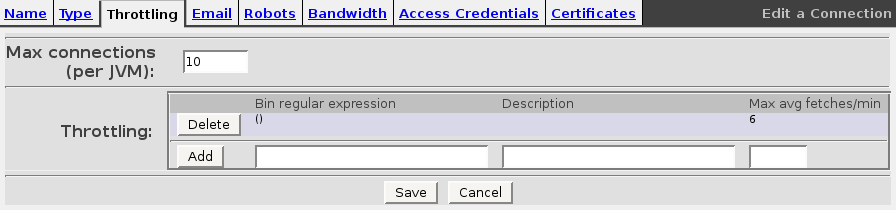
\includegraphics[width=300pt]{web-edit-repository-tab3}

\begin{itemize}

\item \textbf{Max connections (per JVM):} Here you can set the
maximum number of connections to your repository. For the Web Crawler,
you should increase the number of connections from the default 10 to
100. Configuration of other sections on this tab and the ``Bandwidth''
tab allow you to limit the number of connections to individual servers;
increasing the number here helps ensure that the crawler is able to take
full advantage of multiple throttling groups, which are explained below.


\item \textbf{Throttling:} Here you can set a maximum average document fetch
rate for the repository connection. The maximum fetch rate allows you
to set three things: Expression, description, and fetches per minute.

In the Web Crawler, the bin expression for a document is the name of
the server that hosts it. For example, if a document's URL is
\url{http://www.example.com/index.html}, the bin expression
associated with the document is \texttt{www.example.com}.  You can
create regular expressions to match the bin expression. The example
given here, \texttt{()}, matches all expressions, and thus throttles
all documents together. We recommend a maximum average rate of 6
fetches per minute.  Once you have set an expression, description, and
rate, click Add.

% Can you say what the expression is? I can't read it in the picture
% and I even have pretty good eyes :) 

\end{itemize}

In general, you should be conscientious about document fetch rates,
download rates, and other rates related to server traffic when using
the Web Crawler to connect to servers on the open Internet. The
recommended rates suggested in this guide are typically an upper
limit. You should not exceed these suggestions when crawling servers
on the open Internet. Higher demands on these servers may produce
undesirable effects in their performance; the administrators of those
servers may block your connection.

% We capitalize this more often than we don't; I will fix it everywhere.

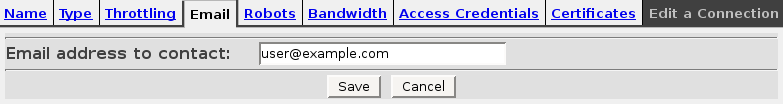
\includegraphics[width=300pt]{web-edit-repository-tab4}

\begin{itemize}

\item \textbf{Email:} A contact email address. This email address is included in request headers sent to servers. Administrators of servers recieving these requests may wish to contact you regarding your interactions with their content servers.

\end{itemize}

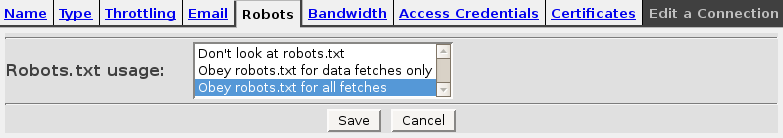
\includegraphics[width=300pt]{web-edit-repository-tab5}

\begin{itemize}

\item \textbf{Robots.txt Usage:} This determines whether the crawler obeys guidelines from the \dirpath{robots.txt} file on a server. There are three options:

\begin{itemize}

\item \textbf{Don't look at robots.txt}

\item \textbf{Obey robots.txt for data fetches only}

\item \textbf{Obey robots.txt for all fetches}

\end{itemize}

By default, \textbf{Obey robots.txt for all fetches} is selected. When
selected, the crawler will obey all interfacing and downloading
guidelines set in a server's \dirpath{robots.txt} file. You should
always use this setting when connecting to servers on the open
Internet.

\end{itemize}

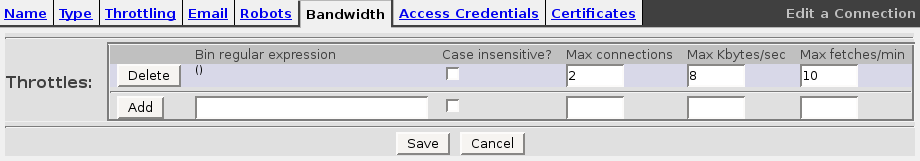
\includegraphics[width=300pt]{web-edit-repository-tab6}

On this tab, you can create throttling groups to limit maximum
connection, download, and fetch rates.

\begin{itemize}


\item \textbf{Throttles}:

\begin{itemize}

\item \textbf{Bin regular expression}: A regular expression to match the bins, as described previously.

\item \textbf{Case insensitive?} Should the match expression be case insensitive?

\item \textbf{Max connections}: The maximum number of connections to for each throttle group. This should be 1 or 2 for servers on the open Internet.

\item \textbf{Max Kbytes/sec}: The maximum download rate for each throttle group. This should be no more than 8 kilobytes per second for servers on the open Internet.

\item \textbf{Max fetches/minute}: The maximum number of document fetches per minute for each throttle group. This should be no higher than 10 fetches per minute for servers on the open Internet.

\end{itemize}

\end{itemize}

The set of all throttle groups you create should cover all the servers
that will be crawled through this repository connection. The easiest
way to ensure that you are limiting all server traffic is to create a
throttling group with the expression \texttt{()} and the appropriate
traffic limits, as shown in the picture above.

\bigimage{web-edit-repository-tab7}


On this tab, you can provide credentials for the crawler to use when
crawling servers protected by basic authentication or NTLM.

\begin{itemize}

\item \textbf{Access Credentials:} 

\begin{itemize}

\item \textbf{URL regular expression}:
Here you can specify a regular expression based on URL. If the crawler
requires credentials when attempting to crawl a document with a
matching URL, it will use the credentials supplied in the following
fields.

\item \textbf{Authorization type}: Select NTLM authentication or basic authentication. (Only LM and NTLMv1 are supported at this time.)

\item \textbf{Domain}: Here you can specify the NTLM domain that will be supplied as part of the user name credentials. Only required if you selected NTLM authentication.

\item \textbf{User name}: The user name that the crawler will use to connect.

\item \textbf{password}: (Optional) The password corresponding with that user name.

\end{itemize}

\end{itemize}

Click the ``Add'' button to include the specified credentials. You can
add multiple sets of credentials.

\missing{The main new feature for this release, see notes in graph paper, will need more screenshots}

\bigimage{web-edit-repository-tab8}

\begin{itemize}

\item \textbf{Trust certificates:}
In some cases, the crawler may need SSL certificates to access certain
content. You can upload SSL certificates here. This is dependent on
the configuration of the servers hosting the crawled content.  The
repository connection will need certificates similar to those used to
connect to the documents using an Internet browser.


If the certificate authority used to sign the content server's
certificate is a well-known authority, you will not need to upload a
certificate here; the appliance will automatically accept a
certificate from the server. If the server certificate is signed by an
unknown authority, you should upload the authority's certificate. In
some cases, the authority may be unavailable. In this case, you can
upload the server-side certificate itself. Server-side certificate
changes may require you to upload newer versions of this certificate
if you use this option.



\end{itemize}

After entering this information, you will be taken to the repository
connection status page for this repository:

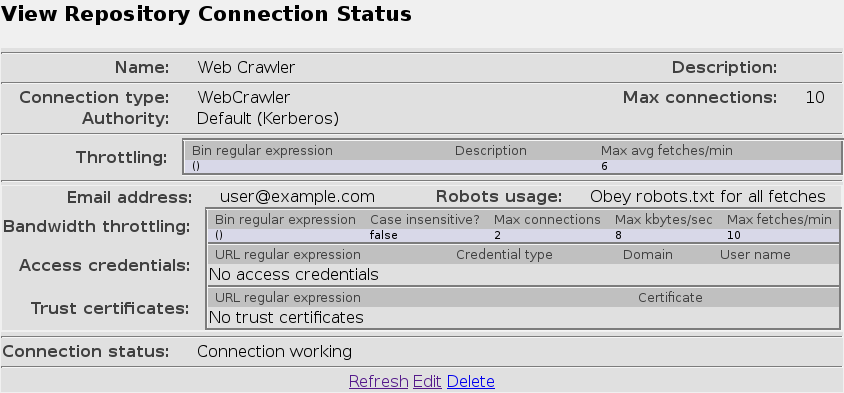
\includegraphics[width=300pt]{web-view-repo-conn-status}

In this example (which does not contain accurate information for any Web
Connector), the Connection Status is ``Connection working.''  If the
Connection Status is ``Connection failed,'' the web sites you want to
crawl might be down. Alternately, you might have incorrectly entered
data in one of the fields; if so, click ``Edit'' to fix the data.
